\documentclass[11pt,letterpaper]{exam}
\usepackage{amsmath}
\usepackage[utf8]{inputenc}
\usepackage[spanish]{babel}
\usepackage{graphicx}
\usepackage{tabularx}
\usepackage[absolute]{textpos} % Para poner una imagen en posiciones arbitrarias
\usepackage{multirow}
\usepackage{float}
\usepackage{hyperref}
\usepackage{breakurl}
\usepackage{multicol}
\decimalpoint

\begin{document}
\begin{center}


\includegraphics[width=16cm]{header.png}

\vspace{1.0cm}
{\Large Herramientas Computacionales - Tarea 7}
2016-II
\end{center}

%\begin{textblock*}{40mm}(10mm,20mm)
%  
\includegraphics[width=3cm]{logoUniandes.png}
%\end{textblock*}

%\begin{textblock*}{40mm}(164mm,20mm)
%  
\includegraphics[width=3cm]{logoUniandes.png}
%\end{textblock*}

\vspace{0.5cm}

\noindent
Los archivo del c\'odigo fuente debe subirse a Sicua plus en un \'unico archivo
\verb".zip" con el nombre del estudiante en el formato \verb"NombreApellido_hw7.zip" antes que termine la clase.

El objetivo de este ejercicio es utilizar arreglos de numpy y las funciones \verb'imshow' e \verb'imread' de matplotlib para analizar una imagen. Debe ser realizado en un notebook de Ipython. Las librer\'ias pueden ser importadas con el comando \verb'%pylab inline'.

\vspace{0.5cm}

\begin{questions}
 
\question[1] {\bf{Importar y mostrar la imagen}}

Descargue la imagen del siguiente enlace: \url{https://www.tutorialspoint.com/dip/images/einstein.jpg} .

\begin{figure}[H]
  \centering
  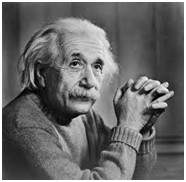
\includegraphics[width=4cm]{einstein}
  %\caption{\label{fig:con-dogma} Procesos involucrados en la expresi\'on gen\'etica.}
\end{figure}

Luego importe la imagen en el notebook, mu\'estrela en escala de grises incluyendo la convenci\'on de colores (\verb'colorbar') e imprima sus dimensiones. Note que adem\'as del largo y ancho de la imagen, hay una dimensi\'on adicional de \verb'3' que corresponde a los valores RGB (Red Green Blue) de cada uno de los pixeles.


\question[1.5] {\bf{Recortar las dimensiones de la imagen}}

Modifique la imagen de tal forma que las dimensiones s\'olamente sean el largo y el ancho de la imagen, es decir, que la nueva imagen sea una matriz donde cada elemento es un n\'umero y no una lista de $3$ elementos como en el caso anterior.

Imprima las dimensiones de la nueva imagen y mu\'estrela en escala de grises incluyendo la \verb'colorbar'. Se deber\'ia ver igual que en el punto anterior. 

\question[1] {\bf{Reflejar la imagen}}

Muestre la imagen reflejada tanto vertical como horizontalmente, las funciones \verb'fliplr' y \verb'flipud' de numpy le pueden ser \'utiles, consulte su documentaci\'on en internet. Se deben ver de la siguiente manera:

\begin{figure}[H]
  \centering
  \includegraphics[width=4cm]{lr}
  %\caption{\label{fig:con-dogma} Procesos involucrados en la expresi\'on gen\'etica.}
\end{figure}
\begin{figure}[H]
  \centering
  \includegraphics[width=4cm]{ud}
  %\caption{\label{fig:con-dogma} Procesos involucrados en la expresi\'on gen\'etica.}
\end{figure}

\question[1.5] {\bf{Invertir la imagen}}

Note que cada elemento (pixel) de la imagen modificada es un valor entre $0$ y $255$. Donde $0$ es negro y $255$ es blanco. Para invertir la imagen, los pixeles m\'as oscuros deben convertirse en los m\'as claros y viceversa.

Muestre la imagen invertida incluyendo la \verb'colorbar'. Debe verse de la siguiente manera:

\begin{figure}[H]
  \centering
  \includegraphics[width=4cm]{inv}
  %\caption{\label{fig:con-dogma} Procesos involucrados en la expresi\'on gen\'etica.}
\end{figure}

\end{questions}

\end{document}
